\documentclass{acm_proc_article-sp-sigmod09}
\usepackage{algorithm2e}

\begin{document}
	
	% --- Author Metadata here ---
	\conferenceinfo{Ambrosi, Andrea \qquad \qquad \qquad \qquad   Toniatti, Carlo}{\\ andrea.ambrosi-1@studenti.unitn.it\quad carlo.toniatti-2@studenti.unitn.it}
	
	\CopyrightYear{2019}
	% --- End of Author Metadata ---
	
	\title{Data mining project: pattern recognition}
	\subtitle{LM Data Science, Data mining}
	
	\author{
		Ambrosi, Andrea\\
		\texttt{[212317]}
		\and
		Toniatti, Carlo\\
		\texttt{[205515]}
	}
	
	\maketitle
	\begin{abstract}
		This report describe the process of pattern recognition used to draw some important rules in order to understand which kind of products are exchanged between cities in a simulated world.
	\end{abstract}
	
	% A category with the (minimum) three required fields
	\category{H.4}{Information Systems Applications}{Miscellaneous}
	%A category including the fourth, optional field follows...
	\category{D.2.8}{Software Engineering}{Metrics}[complexity measures, performance measures]
	
	\terms{Data mining}
	
	\keywords{Data, mining, pattern-recognition} % NOT required for Proceedings
	
	\section{Introduction}
	``The field of pattern recognition is concerned with the automatic discovery of regularities in data through the use of computer algorithms and with the use of these regularities to take actions such as classifying the data into different categories.''\footnote{Bishop, Christopher M. (2006). Pattern Recognition and Machine Learning. Springer.}
	\\
	\\
	Nowadays a lot of applications are producing data records highly interconnected one another where the appearance of a record depends on the appearance of another one. Furthermore, each record is not a black-closed-box item where it is possible to see only the exterior or the result that it produces but consists of a number of characteristics that shape it. The objective of this project is to produce an efficient algorithm for computing the frequent patterns hidden inside the dataset made by the Big Data project work and to have as result a set of informative relationships that link cities and products.
	\\
	\\
	The report is organized in the following way: in the second section we'll talk about the data, the structure of the dataset and the cleaning we did in order to process them. In the third section we'll dive inside the project problem with our interpretation of the job and trying to formalize it. Then in the section four we'll see the solutions we have tried in order to find out recurrent patterns and the tuning of the parameters to refine and speed up the execution.
	
	\section{The data}
	In this part of the work we wanted to have a look to the data generated with the Big data project. As assumption, to be more similar to a real situation, we will treat the data as if the work started at this point so without knowing anything about the structure of the dataset and the origin of what there's inside.
	
	\subsection{Description}
	Let's start with an example that it is possible to find in the Table 1.
	In the dataset generated by the previous work, data are collected in a tabular form so there are 6 columns defining each one an attribute of the record.
	Each record in the dataset is a trip and it is defined by the ``RouteId'' and the ``Order'' that are, in SQL terms, the keys of the table. From the just aforementioned definition, there wont be in the dataset another pair with the same ``(RouteId, Order)'' because each couple defines a different trip. 
	For every trip there is a ``TruckCode'' that identifies the truck that is used to transport the orders, a ``StartCity'' and an ``EndCity'' which identifies the beginning and the conclusion of the trip.
	A route in this dataset is made up of some trips that vary between 3 and 10 cities and each trip brings items between 3 and 15.
	Analyzing the data it is possible to discover that there are almost 100 cities and 150 routes. Considering that more or less every route has between 3 and 10 trip, in average it will produce 700/800 orders (or trips) in the dataset.
	\begin{table*}
		\centering
		\caption{A route example}
		\begin{tabular}{|c|c|c|c|c|p{7cm}|} \hline
			\textbf{RouteId}&\textbf{Order}&\textbf{TruckCode}&\textbf{StartCity}&\textbf{EndCity}&\textbf{Items}\\ \hline
			0&0&18&Allende&Pristina&\{'Blueberry-syrup',
				'Cereales',
				'Chocolate-mousse', [...]\}\\ \hline
			0&1&18&Pristina&Akkol'&\{'Cereales',
				'Chocolate-mousse',
				'Flavoured-cranberries', [...]\}\\ \hline
			0&2&18&Akkol'&Wertheim&\{'Beef-lasagne',
				'Feta-cheese',
				'Flavoured-cranberries', [...]\}\\ \hline
			\end{tabular}
	\end{table*}
	
	\subsection{Cleaning}
	In this section we deviate from the assumption of the real situation of which we know nothing because this would have produced a lot of extra and unnecessary work. In the development of the dataset there are some constraint that let us to relax when analyzing the data. The only few things that have to be taken into account are the way in which the data are stored and the process that have to be adopted for the pattern discovery. According to this problem, a little work have been done in order to prepare the items for the processing so they have been trimmed to delete white spaces and strange characters that appeared in the ``Items'' field such as commas, apostrophes and curly brackets to transform it in a simple list of items.
	As example, the items in Table 1 have been turned from\\
	\{$'Blueberry-syrup',$ $'Cereales',$ $'Chocolate-mousse'$\}\\
	\{$'Cereales',$ $'Chocolate-mousse',$ $'Flavoured-cranberries'$\}\\
	\{$'Beef-lasagne',$ $'Feta-cheese',$ $'Flavoured-cranberries'$\}
	\\to\\
	$[Blueberry-syrup,$ $Cereales,$ $Chocolate-mousse]$\\
	$[Cereales,$ $Chocolate-mousse,$ $Flavoured-cranberries]$\\
	$[Beef-lasagne,$ $Feta-cheese,$ $Flavoured-cranberries]$
	This way it is possible to treat the Items column as a list of lists that is more efficient for the work we have to do later.
	
	\section{The problem}
	
	\subsection{Interpretation}	
	To talk about pattern finding may be easy because there are a lot of examples we can use but it can be tricky and guide to wrong conclusions if no particular care is given to the importance of the relationship discover.
	As we have seen in the Table 1 of the section 2.1, the trips have the form:
	\begin{center}
	$<RouteId,$\quad \quad$Order,$\quad \quad$TruckCode,$\\
	\qquad$StartCity,$\quad$EndCity,$\quad$Items$\quad\qquad$>$
	\end{center}
	What we are interested in, is the sequence of products in different trips, in order to understand which kind of products travel across the system, which cities they meet and what are the frequent items that pass very often between 2 cities or simply which tuples of products appears very often in the dataset.
	
	\subsection{Related works}
	\subsubsection{A priori algorithm}
	The problem of frequent pattern mining is to discover relationships among a set of items within a database: for this reason, it is proper to define a value $t$, defined more in general as support threshold. Thus, if an item appears at least $t$ times, it should be considered as frequent. This is a foundamental concept in Data Mining, and it is central in the market basket problem, in which we are interested in finding frequent groups of items bought together.\\
	Afterwards it is important to proceed step-by-step, with the guarantee that the solution will be built on frequent items, which are derived from other frequent entities too: so, it is fundamental to build, at each step, (k + 1) frequent items which have to come from frequent $k$-patterns. The ``A priori'' approach shows perfectly this type of procedure:
\newcommand{\forcond}{$i=0$ \KwTo $n$}
\SetKwProg{Apriori}{Apriori}{:}{}
	\begin{algorithm}[]
		\SetAlgoLined
		\caption{A priori approach}
		\Apriori{(database D, support t)}{
			Generate frequent patterns for the step 1 and 2 of the algorithm. \tcp{Frequent items and frequent couples}
			$k\leftarrow 2$\\
			\While{$F_k$ is not empty}{
				Generate $C_{k+1}$ by using joins $F_k$.\\
				Prune the solution space.\\
				Generate new candidates in $C_{k+1}$ respecting to the support $t$.\\
				$k\leftarrow k+1$\\
			}
			\KwRet{$\bigcup_{i=1}^{k} F_{i}$}
		}
	\end{algorithm}

	Once the sets are scanned, the frequent items were retrieved, a prune of the solution space is performed and the new frequent item set is added to the total result. In this way, it is assured that all the solutions presented in the resulting set are frequent.\\
	This approach can be easily modified in order to find frequent items during a route, in which new candidates for the solution are created adding the next trip in the route: if it is proven that a new subpattern is frequent, it is stored and will be used in order to have a new frequent solution. This is the basis of the mining algorithm presented in this report: we will see it in detail later.
	The threshold value $t$ is another important aspect in the frequent pattern discovery, therefore it has to be used in order to have a limit that discriminate between what we consider frequent and what we consider occasional: the candidates will be rejected in case they can’t overcome it. Taking the chemistry field as example, the threshold can also be assigned in order to describe the strength of the bonds among some atoms.
	
	\subsubsection{PCY algorithm and improvements}
	The ``A-Priori Algorithm'' is fine as long as the step with the greatest requirement for main memory has enough
	memory that it can be accomplished without moving
	data between disk and main memory.
	This algorithm improves on A-Priori by creating a hash table on the first pass, using all main-memory space that is not needed to count the items. Pairs of items are hashed, and the hash-table basket are used as integer counts of the number of times a pair has hashed to that bucket. Then, on the second pass, we only have to count pairs of frequent items that hashed to a frequent bucket (one whose count is at least the support threshold) on the first pass.
	This is only one of the possibilities to make the ``A priori algorithm'' to work better and don't waste memory. There are other methods like the ``Multistage PCY'' that improve PCY by using several successive hash tables to reduce further the number of candidate pairs. The tradeoff is that Multistage takes more than two passes to find the frequent pairs. 
	Sometimes, we can get most of the benefit of the extra passes of the Multistage Algorithm in a single pass with a variation of PCY that is called the ``Multihash Algorithm''. Instead of using two different hash tables on two successive passes, this method uses two hash functions and two separate hash tables that share main memory on the first pass. The danger is that each hash table has half as many buckets as the one large hash table of PCY. As long as the average count of a bucket for PCY is much lower than the support threshold, we can operate two half-sized hash tables and still expect most of the buckets of both hash tables to be infrequent. Thus, in this situation we might well choose the multihash approach.
	
	\section{Explored solutions}
	Before going in deep with the solutions we adopted and have a look to how good the algorithm perform with different values of parameters, we would like to introduce few theoretical concepts in order to understand why we choose some values for the parameters in the algorithm.\\
	The first concept is the ``\textit{support}'' and we'll se it through an example. In the table 2, are listed 5 rows each one with an ``Id'' and with a list of ``items''. Those are baskets in a supermarket that keep track of what someone is buying. The support for an itemset \textbf{I} is defined as the number of baskets	containing all items in \textbf{I} so in this example, the support for the couple \{Beer, Bread\} is 2.
	Then we find the ``\textit{association rules}'' which simply defines the association between a set of items and another item meaning that usually if we find the set \{$x_1$, $x_2$, $x_3$\} then we are most likely to find also $j$.
	Analyzing a dataset it is possible to find a huge number of associations but we are interested only in those that give us an added value. In order to distinguish between associations, we can introduce the concept of ``\textit{confidence}'' than, going on with the previous example, is the probability of $j$ given $I = {i_1,...,i_k}$ and can be calculated as $$conf(I \rightarrow j) = {support(I \cup j) \over support(I)}$$ 
	A problem with this definition is given by the fact that not all high-confidence rule\begin{table}
		\centering
		\caption{Basket example}
		\begin{tabular}{|l|l|}              \hline
			\textbf{Id}&\textbf{Items}   \\ \hline
			1&{Bread, Coke, Milk}        \\ \hline
			2&{Beer, Bread}              \\ \hline
			3&{Bread, Coke, Diaper, Milk}\\ \hline
			4&{Beer, Bread, Diaper, Milk}\\ \hline
			5&{Coke, Diaper, Milk}       \\ \hline
		\end{tabular}
	\end{table}s are interesting because as example, $X \rightarrow \textit{milk}$ may have high confidence for many itemset $X$ only because milk is purchased very often (independently of $X$). To avoid this situation we can introduce the ``\textit{interest}'' that is, for the rule $I \rightarrow j$, the difference between its confidence and the fraction of baskets that contain $j$: $$interest(I \rightarrow j) = conf(I \rightarrow j) - Pr[j]$$ so from this definition, interesting rules are those with high positive or high negative values.

	Now that we have seen some theoretical concepts we can have a look to how the results change if we move the threshold levels for the support, confidence and interest.\\
	In the figure \ref{fig:support} we compare the support threshold level with the number of items that are considered ``\textit{frequent}''. This can be seen as a filter where we keep track only for those items that appear more than the threshold value $t$. Starting from this point we construct the rest of the frequent pattern considering for the step $s+1$ only those items or tuples that appear in the level $s$ more than the threshold value $t$.
	\begin{figure}[h]
		\caption{Support vs. number of items}
		\centering
		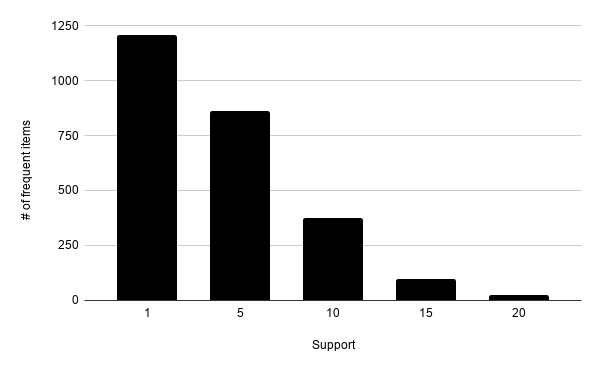
\includegraphics[scale=0.4]{support_items.png}
		\label{fig:support}
	\end{figure}
	\\
	After some tests we decided to keep as support value for the rest of the algorithm $t=5$ that appear to be a good compromise. It produced as result a huge number of items (if we consider the total number that is more or less $1200$) but, considering that the threshold $t$ is the same for every step $s$, we have to keep in mind that in the further steps the tuples are even less and less because of the filtering process so a high threshold would have cause a high number of short pattern and a low number of medium/long pattern.
	
	``\textit{Confidence}'' and ``\textit{interest}'' are the main parameters at this point because a change of these parameters cause the diversification of the pattern in the results.
	As we have seen in the definition, the confidence is important but has to be followed by the interest to have a complete overview of the results. We have done 4 small test in order to gain some information about the behaviour of the algorithm in that situatons:
	\begin{itemize}
		\item $Confidence = 0.3$ and $Interest = 0.3$ \\
		With a low level of confidence our algorithm is going to take into consideration a huge portion of the items and, with also a low level of interest, it won't select interesting rules but it will consider almost all what it encounter. Thus, analayzing the output of the ``\textit{patternExtraction}'' we see that there are a lot of items with few occurrencies for each one.
		\item $Confidence = 0.3$ and $Interest = 0.7$ \\
		In this second test, the low level of confidence as in the previous test, make the algorithm to take into consideration a lot of uninterest items. Nevertheless, with the high level of interest we cut down a lot of useless associations with the result of a quite interesting situation.
		\item $Confidence = 0.7$ and $Interest = 0.3$ \\
		On the other side, with an high level of confidence we fall into the situation described above in the definition of \textit{confidence} with the example of milk: the interesting items are considered but, with a low level of interest are considered interesting also common products so we don't discover anything new.
		\item $Confidence = 0.7$ and $Interest = 0.7$ \\
		In this last test, we avoid the problem described in the last test because the filter is really tight and pass to the step $s+1$ only those that are interesting (so they have an high confidence) and those that are more rare (due to the high interest). The negative side of the coin is that if the threshold are too high only few items/tuples will pass to the next step producing few short (but really interesting) frequent patterns.
	\end{itemize} 
	
	For all the aforementioned reasons we decided to do not tighten too much the filtering process and we finally set the \textit{confidence} and the \textit{interest} to $0.5$ in order to have a great level of filtering without reducing too much the length and the number of patterns.	
	
	\section{Results}
	\subsection{Pattern discovery}
	The results that we have after the execution of the pattern finding section of the program are actually various: there may be a small pattern like:\\ \\
	\null \qquad \qquad $\rightarrow$ Chinese-food \\ \null \qquad \qquad \qquad \qquad 0 $\rightarrow$ Chinese-food\\ \\
	where the pattern is composed by 2 items, the first is the head of the pattern, then we see the $0$ that means that the items that follows are just after the head. This pattern means that in a route we find ``frequently'' \textit{Chinese-food} in one of the trip and \textit{Chinese-food} in the trip that follows. This can be explained by the fact that a product may be on the truck and it has to travel from $A$ to $C$ but in the middle it has to pass also from $B$.\\
	Then there may be longer pattern like:\\ \\
		\null \qquad \qquad $\rightarrow$ Mint-jelly \\ 
		\null \qquad \qquad \qquad 0 $\rightarrow$ Cigarettes\\
		\null \qquad \qquad \qquad 0 $\rightarrow$ Mint-jelly\\
		\null \qquad \qquad \qquad \qquad 1 $\rightarrow$ Assortiment-de-fromages\\
		\null \qquad \qquad \qquad \qquad 1 $\rightarrow$ Mint-jelly\\
		\null \qquad \qquad \qquad \qquad \qquad 2 $\rightarrow$ Frozen-peas\\
		\null \qquad \qquad \qquad \qquad \qquad \qquad 3 $\rightarrow$ Raw\\
		\null \qquad \qquad \qquad \qquad 1 $\rightarrow$ Frozen-peas\\
		\null \qquad \qquad \qquad \qquad \qquad 2 $\rightarrow$ Raw\\ \\
	where after an order that store the head \textit{Mint-jelly} we find ``frequently'' trips that contains \textit{Cigarettes} or \textit{Mint-jelly} and this last one is ``frequently'' followed by trips with \textit{Assortiment-de-fromages}, \textit{Mint-jelly} and so on.\\ \\ \\ \\ \\
	Analyzing the outputs it may be the case that comes out pattern like this one:\\ \\
	\null \qquad \qquad $\rightarrow$ Chocolate-chunks\\
	\null \qquad \qquad \qquad 0 $\rightarrow$ Chocolate-chunks, Dolminades \\
	\null \qquad \qquad \qquad \qquad \qquad 2 $\rightarrow$ Red-ale, Biskuvi\\ \\
	This last example seems to be a strange one but it actually represents the situation where we find something frequent in an order, in the successive one there's anything frequent while after some steps something interest comes out. If this structure appear frequently we mark it as frequent also if there are holes in the middle.
	To make it more clear we want to describe better how the output is structured: in the first position, after the right arrow we find the head of the pattern. In the next rows there are numbers followed by right arrows and then one or more products. The numbers are intended to be the step after the head of the pattern so in the first example we find usually \textit{Chinese-food} after an order that contains \textit{Chinese-food}. In the second example, the pattern become a little more complicated: there are $2$ levels $0$. The $2$ situations that comes out from that pattern are in one case a trip that carry \textit{Mint-jelly} that is frequently followed by a trip with \textit{Cigarettes} and in the other case there is a trip that carry \textit{Mint-jelly} that have also in the following trip \textit{Mint-jelly} and in the successive trip it can carry \textit{Assortiment-de-fromages} or \textit{Mint-jelly} ecc.
	This situation can be better visualize with the help of a tree like in figure \ref{fig:tree}:
	\begin{figure}[h]
		\caption{Tree visualization of a pattern}
		\centering
		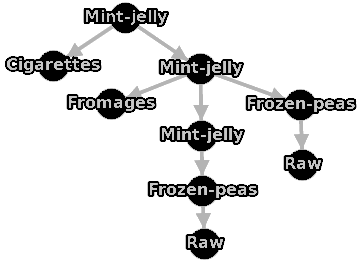
\includegraphics[scale=0.4]{tree.png}
		\label{fig:tree}
	\end{figure}

	The tree visualization explain better what we mean here for pattern so actually with one tree like the one in figure \ref{fig:tree} we can define 4 different paths that start with the same root.
	\subsection{The join with the cities}
	After the pattern discovery section, we decided to investigate the information that a dataset like the one used in this project would provide with some more analysis.
	One of the ideas we had looking at the data was: we have a dataset that store information about all the cities that are traveled by the products and we know what are the frequent pattern of products that can be found in a route. Why don't we join them? With this idea we produced the algorithm \ref{algo:link} that is full of controls and actually is the main time consuming part of the project because it has to pass through all the items, the trips, and the routes for all the patterns discovered it require a lot of time.
	
	\begin{algorithm}[]
		\SetAlgoLined
		initialize \textit{foundInRoute} \\
		\ForEach{route in routes}{
			\ForEach{trip in route}{
				\ForEach{pattern in patterns}{
					\If{head of the pattern is in trip}{
						\If{pattern is not longer than the route}{
							\ForEach{level of pattern}{
								\ForEach{tuple in level}{
									\If{tuple is in the current trip}{
										Add the tuple into foundInRoute  the position given by [startCity][endCity] with the current level
									}
								}
							}
						}
					}	
				}	
			}
		}
		\label{algo:link}
		\caption{Algorithm for linking frequent patterns and cities}
	\end{algorithm}
	\newpage
	The results produced by the algorithm \ref{algo:link} are of the form:\\ \\
	\null \qquad \{('Brescia', 'Verona'): \\
	\null \qquad \qquad \qquad 0: \{('Biscotti',), ('Caramel-popcorn',)\}, \\
	\null \qquad \qquad \qquad 1: \{('Biscotti',), ('Orange-juice', 'Tortilla')\}, \\
	\null \qquad \qquad \qquad 2: \{('Chili-con-carne',), ('Epices',), ('Tarts',)\}, \\
	\null \qquad \qquad \qquad 3: \{('Soda',), ('Fish-sauce',), ('Tarts',)\}, \\
	\null \qquad \qquad \qquad 4: \{('Soda',), ('Fish-sauce',)\\
	\null \qquad\}\\ \\
	where for every couple of cities there can be found at level $0$ the products that travel frequently between those cities, at level $1$ the products that are seen frequently in one step after the city of arrive and so on.
	
	\section{Conclusions and \\further developments}
	To sum up, we started with a dataset generated by the previous work of big data where we had to design a pseudo-random dataset introducing some dependencies. Then with this project the aim was to discover the frequent pattern hidden into the dataset. To make this work we started analyzing the items into each trip and then with a sort of an ``\textit{A priori}'' algorithm we went through all the routes selecting firstly the frequent items then the frequent couples based on the frequent items and so on.\\ 
	After this job of pattern finding, we developed an algorithm in order to analyze the dataset from a different perspective. This solution permitted us to produce a list of couples of cities with for each of them the list of frequent products that travel from one to the other and towards the successive cities.\\
	Into this project there are surely some parts that might be improved and developed more deeply. One of the point that might need some work is the $patternExtraction$ because it is one of the bottleneck in our code. Another algorithm that need some improvement is the algorithm \ref{algo:link} that is really time consuming. In this case a solution based on the dynamic programming should be really useful because in that way a lot of duplicates would be avoided. Once again for the algorithm \ref{algo:link}, the solution might become more clear if, after the frequent products between the 2 cities, the products in the following levels were treated as products for different cities and not simply all toghether for the next levels.
\end{document}
